
\section{Ap\^endice - Modelos ARIMAX (7,1,7), SARIMA (7,1,7) (2,1,0,12) e SARIMAX (7,1,7) (2,1,0,12) 24h}\label{sec:arimaxsarimasarimax24}

\begin{figure}[H]
	\centering
	\caption{Comparação dos modelos ARIMAX, SARIMA e SARIMAX, 1 dia à frente }
	\label{fig:1-ARIMAX-SARIMA-SARIMAX24}
	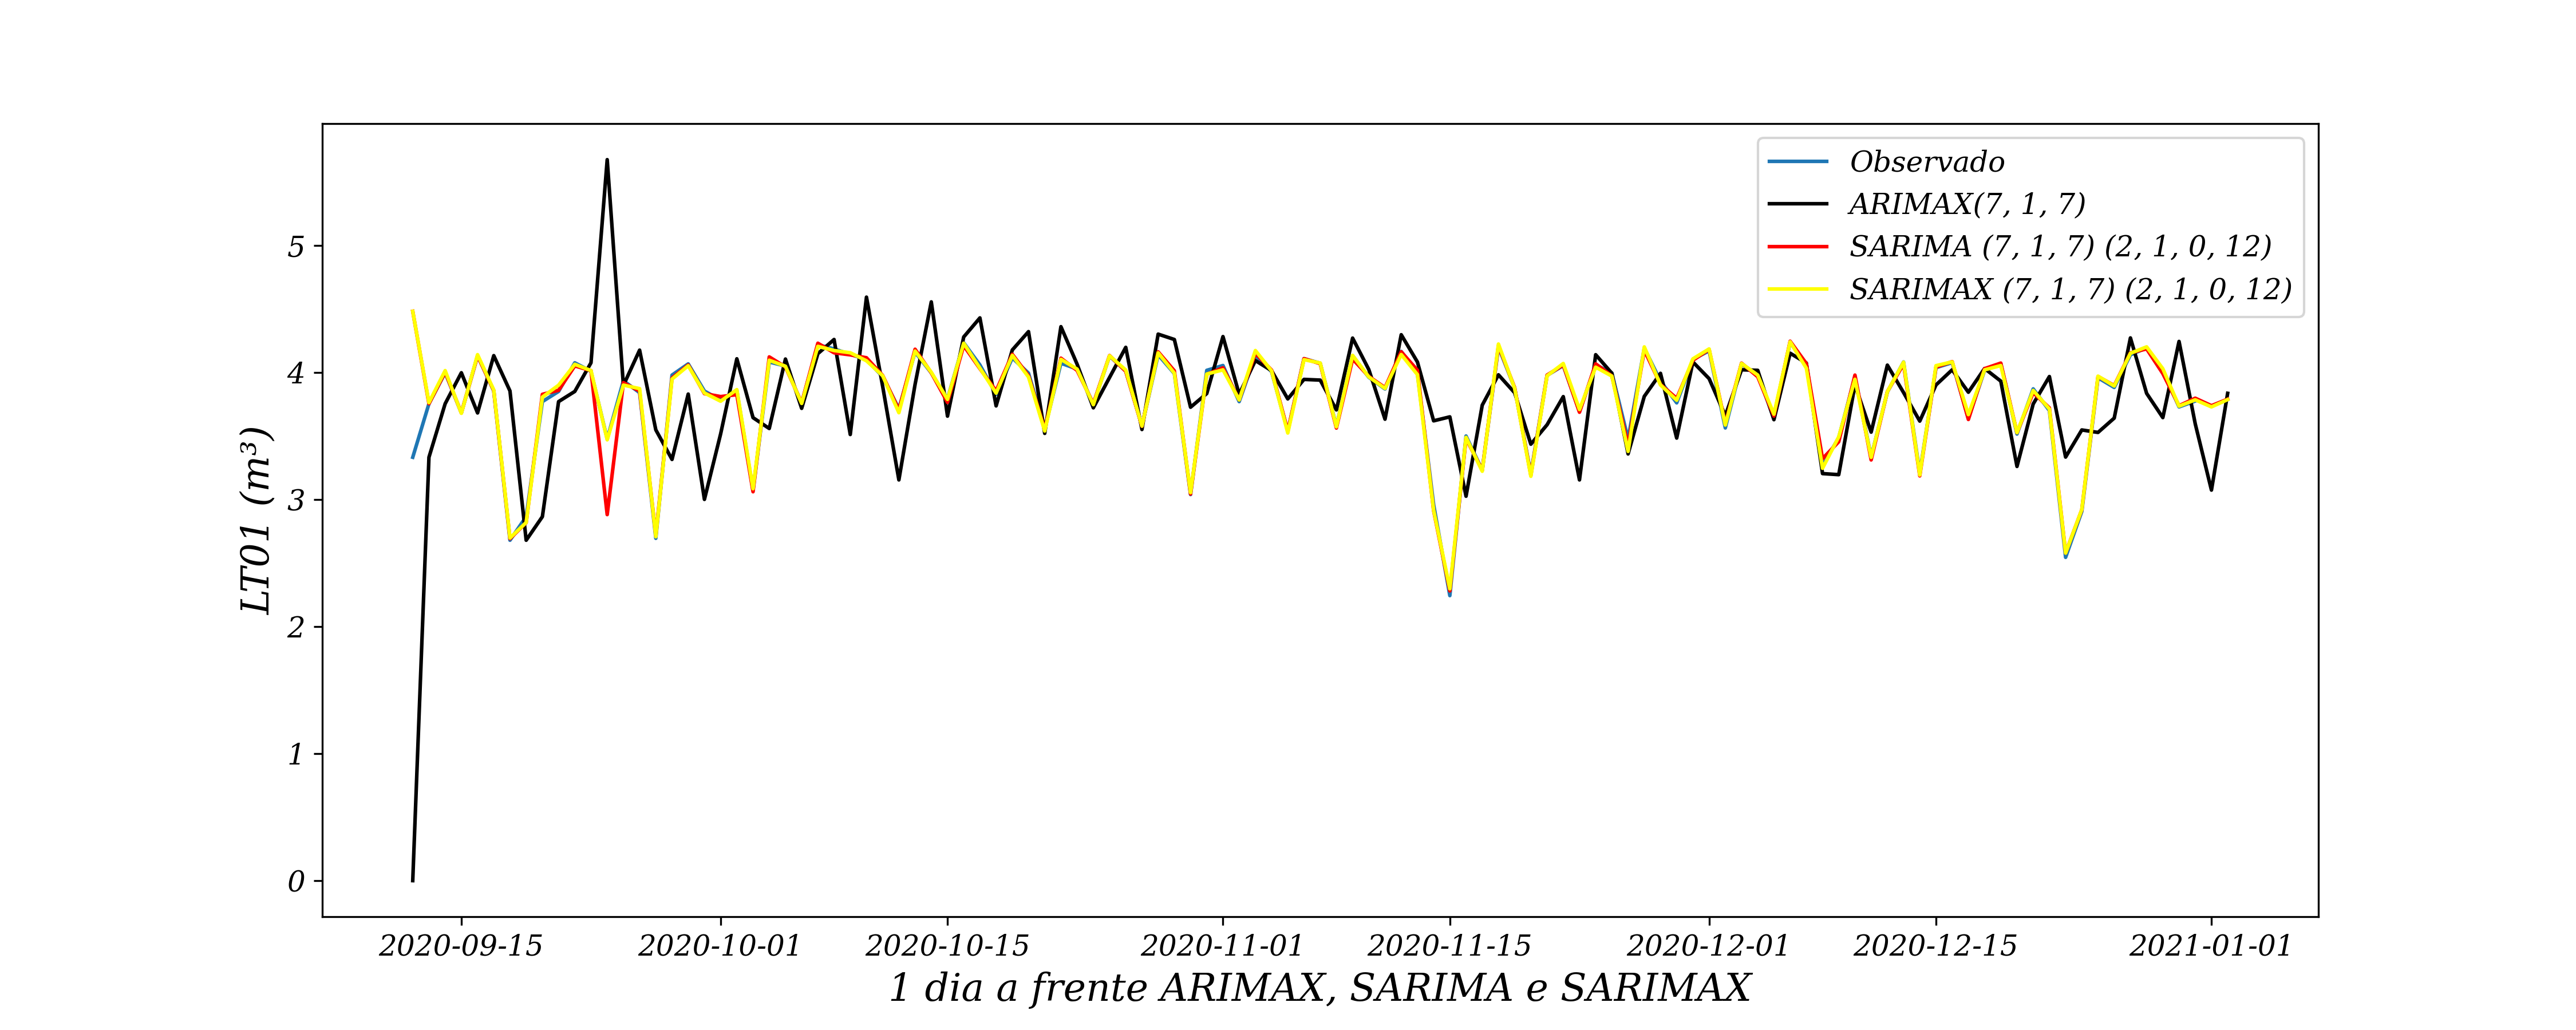
\includegraphics[width=1\linewidth]{Apendices/Figuras/modelagem-24h/1-ARIMAX-SARIMA-SARIMAX}
	
		\fonte{Elaboração própria a partir de dados da SANEPAR (2018 a 2020)}
\end{figure}

\begin{figure}[H]
	\centering
	\caption{Comparação dos modelos ARIMAX, SARIMA e SARIMAX, 7 dias à frente }
	\label{fig:10-ARIMAX-SARIMA-SARIMAX24}
	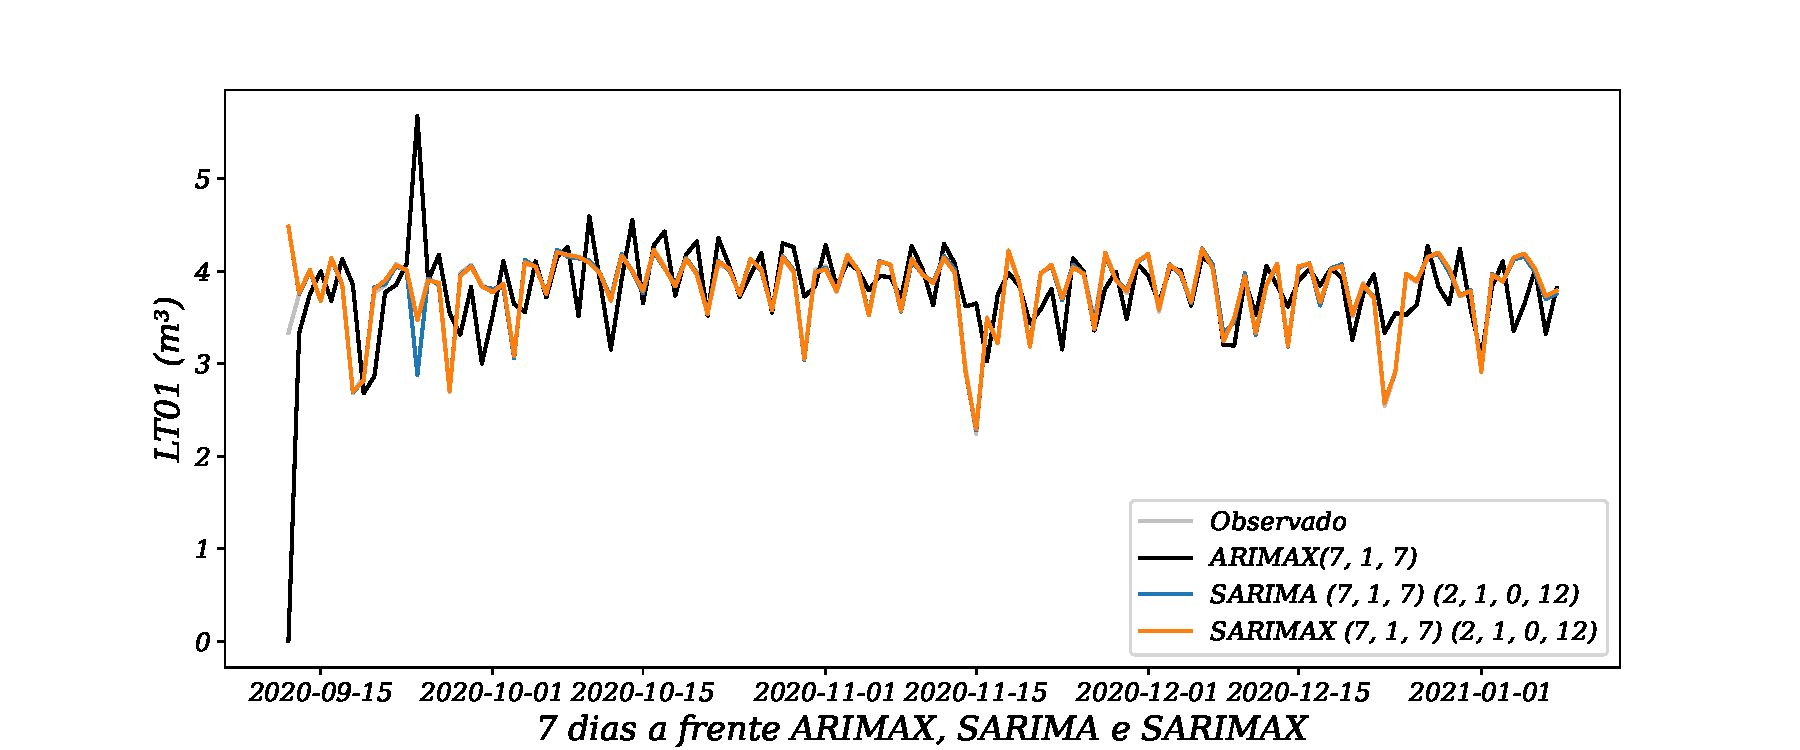
\includegraphics[width=1\linewidth]{Apendices/Figuras/modelagem-24h/7-ARIMAX-SARIMA-SARIMAX}
	
	\fonte{Elaboração própria a partir de dados da SANEPAR (2018 a 2020)}
\end{figure}


\begin{figure}[H]
	\centering
	\caption{Comparação dos modelos ARIMAX, SARIMA e SARIMAX, 14 dias à frente }
	\label{fig:30-ARIMAX-SARIMA-SARIMAX24}
	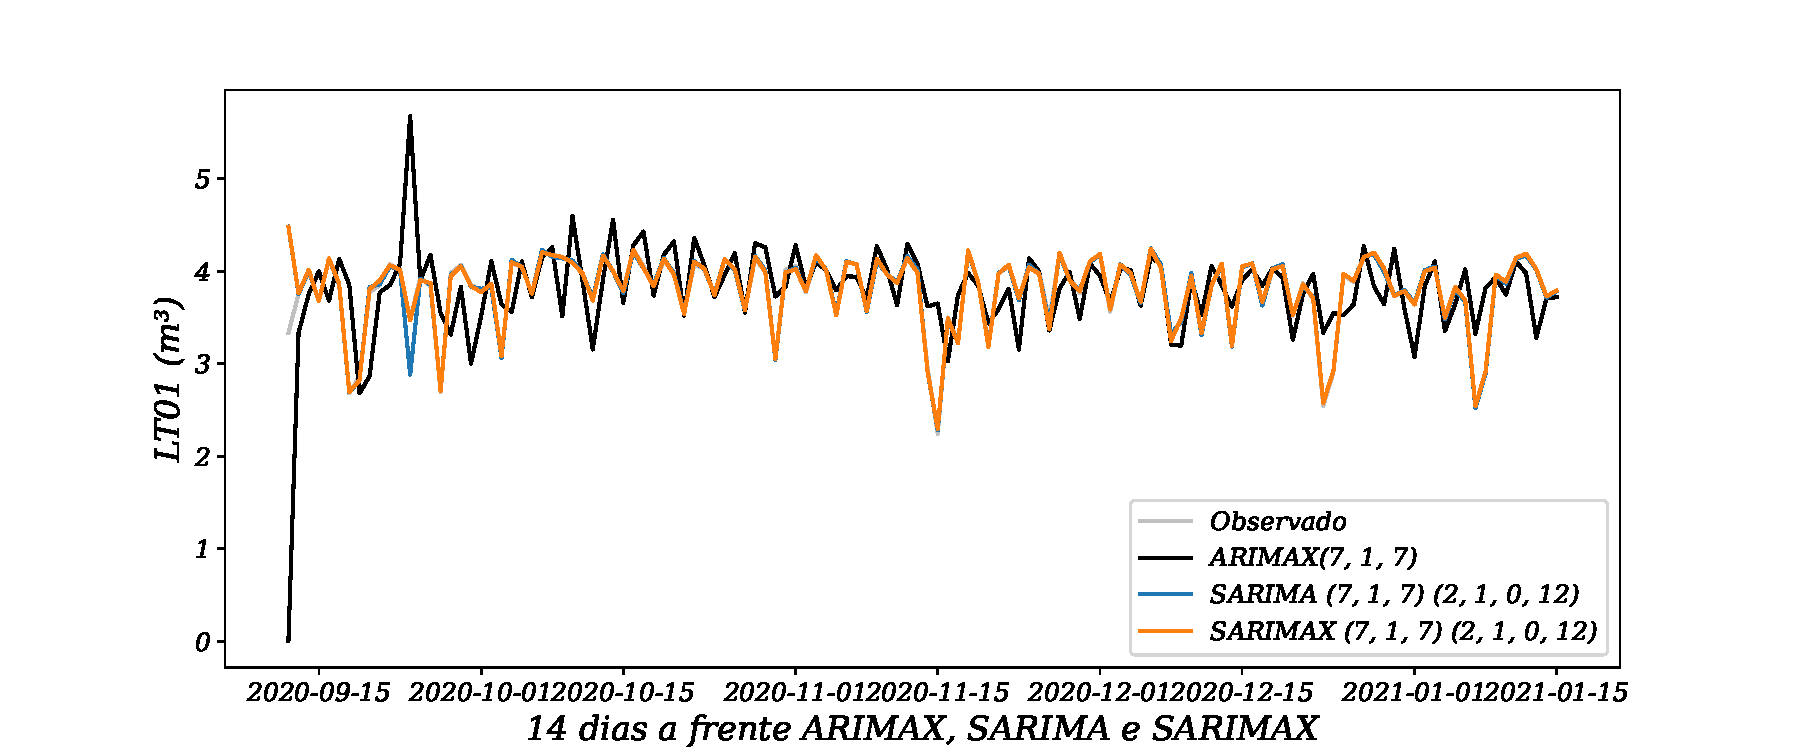
\includegraphics[width=1\linewidth]{Apendices/Figuras/modelagem-24h/14-ARIMAX-SARIMA-SARIMAX}
	
	\fonte{Elaboração própria a partir de dados da SANEPAR (2018 a 2020)}
\end{figure}

\begin{figure}[H]
	\centering
	\caption{Comparação dos modelos ARIMAX, SARIMA e SARIMAX, 30 dias à frente }
	\label{fig:60-ARIMAX-SARIMA-SARIMAX24}
	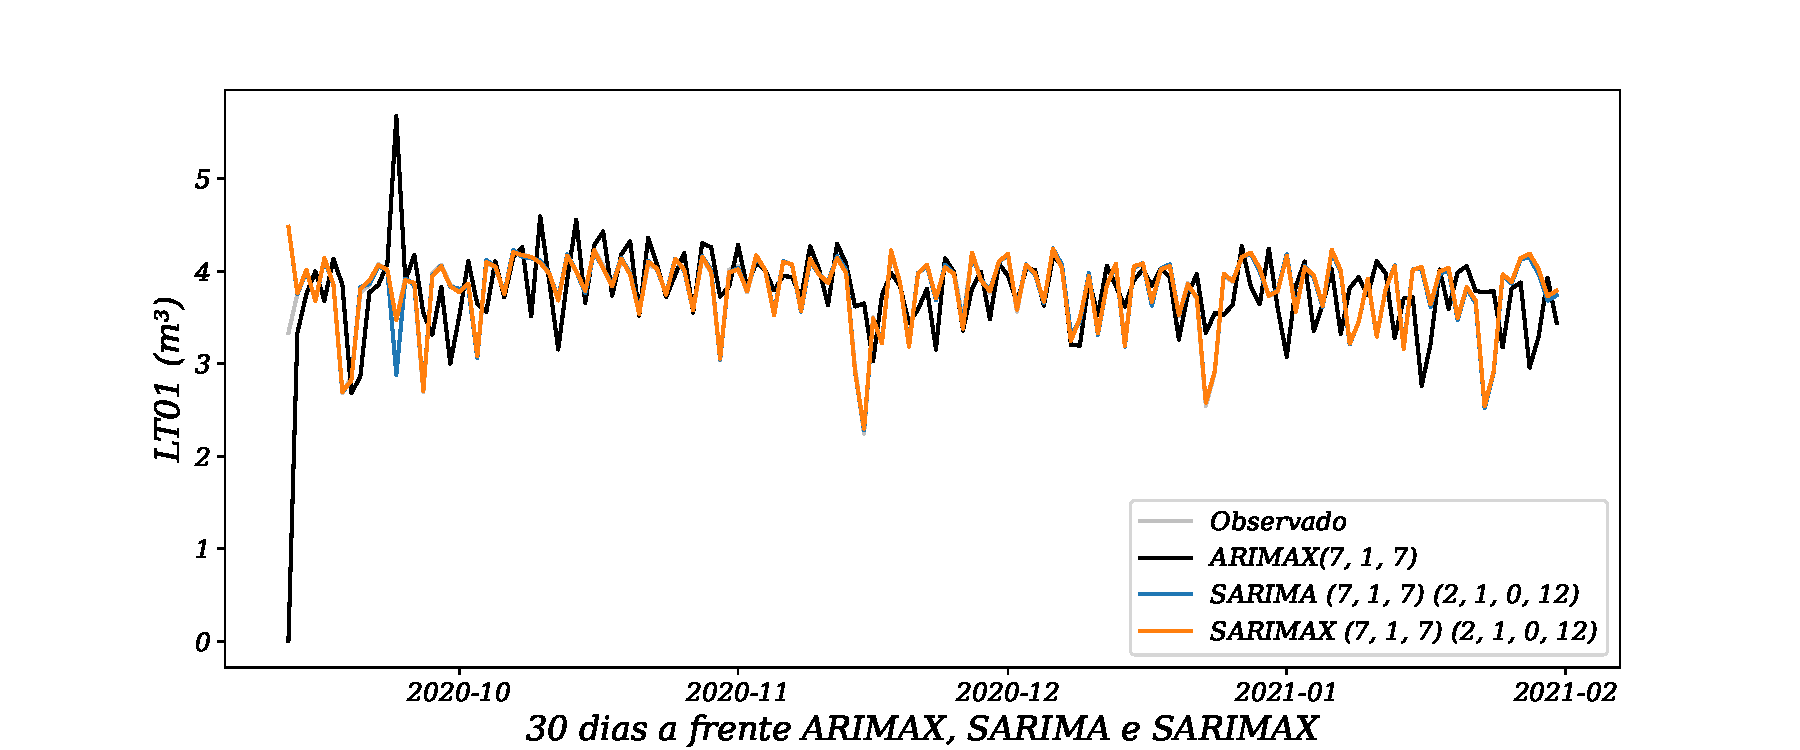
\includegraphics[width=1\linewidth]{Apendices/Figuras/modelagem-24h/30-ARIMAX-SARIMA-SARIMAX}
	
	\fonte{Elaboração própria a partir de dados da SANEPAR (2018 a 2020)}
\end{figure}